% !TeX root = main.tex

\chapter{Introduction}
\glsresetall
\label{chapter:introduction}
\section{High-level Synthesis (HLS)}

The hardware design process has evolved significantly over the years. When the circuits were small, hardware designers could more easily specify every transistor, how they were wired together, and their physical layout. Everything was done manually. As our ability to manufacture more transistors increased, hardware designers began to rely on automated design tools to help them in the process of creating the circuits. These tools gradually become more and more sophisticated and allowed hardware designers to work at higher levels of abstraction and thus become more efficient. Rather than specify the layout of every transistor, a hardware designer could instead specify digital circuits and have \gls{eda} tools automatically translate these more abstract specifications into a physical layout. 

The Mead and Conway approach \cite{mead1980introduction} of using a programming language (e.g., Verilog or VHDL) that compiles a design into physical chips took hold in the 1980s. Since that time, the hardware complexity has continued to increase at an exponential rate, which forced hardware designers to move to even more abstract hardware programming languages. \gls{rtl} was one step in abstraction, enabling a designer to simply specify the registers and the operations performed on those registers, without considering how the registers and operations are eventually implemented. \gls{eda} tools can translate \gls{rtl} specifications into a digital circuit model and then subsequently into the detailed specification for a device that implements the digital circuit.  This specification might be the files necessary to manufacture a custom device or might be the files necessary to program an off-the-shelf device, such as an \gls{fpga}. Ultimately, the combination of these abstractions enables designers to build extraordinarily complex systems without getting lost in the details of how they are implemented.  A non-technical perspective on the value of these abstractions can be found in \cite{lee2017plato}.

 \gls{hls} is yet another step in abstraction that enables a designer to focus on larger architectural questions rather than individual registers and cycle-to-cycle operations.  Instead a designer captures behavior in a program that does not include specific registers or cycles and an \gls{hls} tool creates the detailed \gls{rtl} micro-architecture.  One of the first tools to implement such a flow was based on behavioral Verilog and generated an \gls{rtl}-level architecture also captured in Verilog\cite{knapp96bc}.  Many commercial tools now use C/C++ as the input language.  For the most part the language is unimportant, assuming that you have a tool that accepts the program you want to synthesize!

Fundamentally, algorithmic HLS does several things automatically that an RTL designer does manually:
\begin{itemize}
\item \gls{hls} analyzes and exploits the concurrency in an algorithm.
\item \gls{hls} inserts registers as necessary to limit critical paths and achieve a desired clock frequency.
\item \gls{hls} generates control logic that directs the data path.
\item \gls{hls} implements interfaces to connect to the rest of the system.
\item \gls{hls} maps data onto storage elements to balance resource usage and bandwidth.
\item \gls{hls} maps computation onto logic elements performing user specified and automatic optimizations to achieve the most efficient implementation.
\end{itemize}

Generally, the goal of \gls{hls} is to make these decisions automatically based upon user-provided input specification and design constraints.  However, \gls{hls} tools greatly differ in their ability to do this effectively.  Fortunately, there exist many mature HLS tools (e.g., Xilinx \VHLS, LegUp \cite{canis2011legup}, and Mentor Catapult HLS) that can make these decisions automatically for a wide range of applications. We will use \VHLS as an exemplar for this book; however, the general techniques are broadly applicable to most HLS tools though likely with some changes in input language syntax/semantics. %Note, however, that these capabilities focus primarily on the portions of the RTL design process that are repetitive or common from design to design.  

In general, the designer is expected to supply the \gls{hls} tool a functional specification, describe the interface, provide a target computational device, and give optimization directives. More specifically, \VHLS requires the following inputs:
\begin{itemize}
\item A function specified in C, C++, or SystemC 
\item A design testbench that calls the function and verifies its correctness by checking the results.
\item A target FPGA device
\item The desired clock period
\item Directives guiding the implementation process
\end{itemize}

In general, \gls{hls} tools can not handle any arbitrary software code. Many concepts that are common in software programming are difficult to implement in hardware. Yet, a hardware description offers much more flexibility in terms of how to implement the computation. It typically requires additional information to be added by the designers (suggestions or \lstinline|#pragmas|) that provide hints to the tool about how to create the most efficient design. Thus, \gls{hls} tools simultaneously limit and enhance the expressiveness of the input language. For example, it is common to not be able to handle dynamic memory allocation. There is often limited support for standard libraries. System calls are typically avoided in hardware to reduce complexity. The ability to perform recursion is often limited. On the other hand, \gls{hls} tools can deal with a variety of different interfaces (direct memory access, streaming, on-chip memories). And these tools can perform advanced optimizations (pipelining, memory partitioning, bitwidth optimization) to create an efficient hardware implementation. 

We make the following assumptions about the input function specification, which generally adheres to the guidelines of the \VHLS tool:
\begin{itemize}
\item No dynamic memory allocation (no operators like \lstinline|malloc()|, \lstinline|free()|, \lstinline|new|, and \lstinline|delete()|)
\item Limited use of pointers-to-pointers (e.g., may not appear at the interface)
\item System calls are not supported (e.g., \lstinline|abort()|, \lstinline|exit()|, \lstinline|printf()|, etc. They can be used in the code, e.g., in the testbench, but they are ignored (removed) during synthesis.
\item Limited use of other standard libraries (e.g., common \lstinline|math.h| functions are supported, but uncommon ones are not)
\item Limited use of function pointers and virtual functions in C++ classes (function calls must be compile-time determined by the compiler).
\item No recursive function calls.
\item The interface must be precisely defined.
\end{itemize}

The primary output of an \gls{hls} tool is a \gls{rtl} hardware design that is capable of being synthesized through the rest of the hardware design flow. Additionally, the tool may output testbenches to aid in the verification process. Finally, the tool will provide some estimates on resource usage and performance.  \VHLS generates the following outputs:
\begin{itemize}
\item Synthesizable Verilog and VHDL
\item RTL simulations based on the design testbench
\item Static analysis of performance and resource usage
\item Metadata at the boundaries of a design, making it easier to integrate into a system.
\end{itemize}

Once an \gls{rtl}-level design is available, other tools are usually used in a standard \gls{rtl} design flow.  In the Xilinx \vivado Design Suite, \gls{synth} is performed, translating the \gls{rtl}-level design into a \gls{netlist} of primitive \gls{fpga} logical elements.  The \gls{netlist} (consisting of logical elements and the connections between them) is then associated with specific resources in a target device, a process called \gls{par}.  The resulting configuration of the \gls{fpga} resources is captured in a \gls{bitstream}, which can be loaded onto the FPGA to program its functionality.  The \gls{bitstream} contains a binary representation of the configuration of each \gls{fpga} resource, including logic elements, wire connections, and on-chip memories. A large Xilinx UltraScale FPGAs will have over 1 billion configuration bits and even the ``smaller'' devices have hundreds of millions of bits \cite{ultrascaleArchConfig}. 

%\note{add figure that provides an overview of the hardware design process?}

\section{FPGA Architecture}

It is important to understand the modern FPGA architectures since many of the \gls{hls} optimizations specifically target these features. Over the decades, FPGAs have gone from small arrays of programmable logic and interconnect to massive arrays of programmable logic and interconnect with on-chip memories, custom data paths, high speed I/O, and microprocessor cores all co-located on the same chip. In this section, we discuss the  architectural features that are relevant to \gls{hls}. It is not our intention (nor do we think it is necessary) to provide substantial details of the FPGA architecture. Rather we aim to give the reader enough information to understand the \gls{hls} reports and successfully use and leverage the \gls{hls} directives, many of which very specifically target modern FPGA architectural features.

\glspl{fpga} are an array of programmable logic blocks and memory elements that are connected together using programmable interconnect. Typically these logic blocks are implemented as a \gls{lut} -- a memory where the address signal are the inputs and the outputs are stored in the memory entries. An $n$-bit \gls{lut} can be programmed to compute any $n$-input Boolean function by using the function's truth table as the values of the \gls{lut} memory. 

Figure \ref{fig:lut} a) shows a 2 input \gls{lut}. It has $2^2 = 4$ configuration bits. These bits are the ones that are programmed to determine the functionality of the \gls{lut}.  Figure \ref{fig:lut} b) shows the truth table for a 2 input AND gate. By using the four values in the ``out'' column for configuration bits 0-3, we can program this 2 input LUT to be a 2 input AND gate. The functionality is easily changed by reprogramming the configuration bits. This is a flexible and fairly efficient method for encoding smaller Boolean logic functions. Most \glspl{fpga} use a \glspl{lut} with 4-6 input bits as their base element for computation. Larger \glspl{fpga} can have millions of these programmable logic elements.

\begin{figure}
\centering
\includegraphics[width= \textwidth]{images/lut}
\caption{Part a) shows a 2 input \gls{lut}, i.e., a 2-LUT. Each of the four configuration bits can be programmed to change the function of the 2-LUT making it a fully programmable 2 input logic gate. Part b) provides a sample programming to implement an AND gate.  The values in the ``out'' column from top to bottom correspond directly to configuration bits 0 through 3. Part c) shows a simple \gls{slice} that contains a slightly more complex 3-LUT with the possibility of storing the output into a \gls{ff}. Note that there are nine configuration bits: eight to program the 3-LUT and one to decide whether the output should be direct from the 3-LUT or the one stored in the \gls{ff}. More generally, a \gls{slice} is defined as a small number of \glspl{lut} and \glspl{ff} combined with routing logic (multiplexers) to move inputs, outputs, and internal values between the \glspl{lut} and \glspl{ff}.}
\label{fig:lut}
\end{figure}

\begin{exercise}
How would you program the 2-LUT from Figure \ref{fig:lut} to implement an XOR gate? An OR gate? How many programming bits does an $n$ input ($n$-LUT) require?
\end{exercise}

\begin{exercise}
How many unique functions can a 2-LUT be programmed to implement? How many unique functions can a $n$ input ($n$-LUT) implement? 
\end{exercise}

The \gls{ff} is the basic memory element for the \gls{fpga}. They are typically co-located with a \glspl{lut}. \gls{lut}s can be replicated and combined with \glspl{ff} and other specialized functions (e.g., a full adder) to create a more complex logic element called a configurable logic block (CLB), logic array block (LAB), or \gls{slice} depending on the vendor or design tool. We use the term \gls{slice} since it is the resource reported by the \VHLS tool.  A \gls{slice} is a small number of \glspl{lut}, \glspl{ff} and multiplexers combined to make a more powerful programmable logic element. The exact number and combination of  \glspl{lut}, \glspl{ff} and multiplexers varies by architecture, but generally a slice has only few of each of these elements. Figure \ref{fig:lut} c) shows a very simple slice with one 3-LUT and one FF. A \gls{slice} may also use some more complex logic functions. For example, it is common to embedded a full adder into a slice. This is an example of ``hardening'' the FPGA; this full adder is not programmable logic -- it can only be used as a full adder, but it is common to use full adders (to make addition operations) and it is more efficient to use the custom full adder as opposed to implementing a full adder on the programmable logic (which is also an option). And thus, overall it is beneficial to have a hard full adder in the slice.

Programmable interconnect is the other key element of an FPGA. It provides a flexible network of wires to create connections between the slices. The inputs and outputs of the \gls{slice} are connected to a \gls{routingchannel}. The \gls{routingchannel} contains a set configuration bits can be programmed to connect or disconnect the inputs/outputs of the \gls{slice} to the programmable interconnect. Routing channels are connected to \glspl{switchbox}. A \gls{switchbox} is a collection of switches that are implemented as pass transistors. These provide the ability to connect the routing tracks from one \glspl{routingchannel} to another. 

Figure \ref{fig:slice_channel} provides an example of how a \gls{slice}, \gls{routingchannel}, and \gls{switchbox} are connected. Each input/output to the \gls{slice} can be connected to one of many routing tracks that exist in a routing channel. You can think of routing tracks as single bit wires. The physical connections between the slice and the routing tracks in the routing channel are configured using a pass transistor that is programmed to perform a connect or disconnect from the input/output of the slice and the programmable interconnect. 

\begin{figure}
\centering
\includegraphics[width= 0.8\textwidth]{images/slice_channel}
\caption{ A \gls{slice} contains a small number of \glspl{lut} and \gls{ff}. We show a very simple \gls{slice} with one \gls{lut} and one \gls{ff} though generally these have two or more of each. Slices are connected to one another using a \gls{routingchannel} and \gls{switchbox}. These two provide a programmable interconnect that provide the data movement between the programmable logic elements (\glspl{slice}). The \gls{switchbox} has many switches (typically implemented as pass transistors) that allow for arbitrary wiring configurations between the different routing tracks in the routing tracks adjacent to the switchbox. }
\label{fig:slice_channel}
\end{figure}

The \glspl{switchbox} provides a connection matrix between routing tracks in adjacent \glspl{routingchannel}. Typically, an \gls{fpga} has a logical 2D representation. That is, the \gls{fpga} is designed in a manner that provides a 2D abstraction for computation. This is often called an ``island-style'' architecture where the \glspl{slice} represent ``logic islands'' that are connected using the \glspl{routingchannel} and \glspl{switchbox}. Here the \gls{switchbox} connects to four \glspl{routingchannel} to the north, east, south, and west directions. The exact programming of the switches in the \glspl{routingchannel} and \glspl{switchbox} determines how the inputs and outputs of the programmable logic blocks are connected. The number of channels, the connectivity of the switchboxes, the structure of the slice, and other logic and circuit level FPGA architectural techniques are very well studied; we refer the interested reader to the following books and surveys on this topic for more information \cite{brown1996fpga, betz1997vpr, hauck2010reconfigurable}. Generally, it is not necessary to understand all of the nitty-gritty details of the FPGA architecture in order to successfully use the \gls{hls} tools, rather it is more important to have a general understanding of the various FPGA resources and how the \gls{hls} optimizations effect the resource usage.

\begin{figure}
\centering
\includegraphics[width= 0.7\textwidth]{images/fpga}
\caption{ The two-dimensional structure of an \gls{fpga} showing an island style architecture. The logic and memory resources in the \glspl{slice} are interconnected using \glspl{routingchannel} and \glspl{switchbox}. The input/output (I/O) blocks provide an external interface, e.g., to a memory, microprocessor, sensor, and/or actuator. On some FPGAs, the I/O directly connects to the chip pins. Other FPGAs use the I/O to connect the programmable logic fabric to on-chip resources (e.g., a microprocessor bus or cache).   }
\label{fig:fpga}
\end{figure}

Figure \ref{fig:fpga} provides an even more abstract depiction of an \gls{fpga} programmable logic and interconnect. This provides a larger view of the 2D dimensional layout of the programmable logic (e.g., \glspl{slice}), \glspl{routingchannel}, and \glspl{switchbox}. The \gls{fpga} programmable logic uses \glspl{ioblock} to communicate with an external device. This may be a microcontroller (e.g., an on-chip ARM processor using an AXI interface), memory (e.g., an on-chip cache or an off-chip DRAM memory controller), a sensor (e.g., an antenna through an A/D interface), or a actuator (e.g., a motor through an D/A interface). More recently, \glspl{fpga} have integrated custom on-chip I/O handlers, e.g., memory controllers, transceivers, or analog-to-digital (and vice versa) controllers directly into the fabric in order to increase performance.

As the number of transistors on the FPGA has continued to increase, FPGA architectures have begun to incorporate more and more ``hard'' resources. These are custom resources designed specifically to perform a task. For example, many applications make heavy use of addition and multiplication operations. Thus, the FPGA fabric added custom resources targeted at these operations. An example of this is the DSP48 custom datapaths, which efficiently implement a series of arithmetic operations including multiplication, addition, multiply-accumulate, and word level logical operations. These DSP48 blocks have some programmability, but are not as flexible as the programmable logic. Yet, implementing a multiply or MAC operation on these DSP48s is much more efficient than performing the same operation on the programmable logic. Thus, there is a fundamental tradeoff of efficiency versus flexibility. Modern FPGAs will have hundreds to thousands of these DSP48 distributed throughout the logic fabric as shown in Figure \ref{fig:heterogenous_fpga}.

\begin{exercise}
Compare the performance of a multiply accumulate operation using the programmable logic versus the DSP48s. What is the maximum frequency that one can obtain in both cases? How does the FPGA resource usage change?
\end{exercise} 

\begin{figure}
\centering
\includegraphics[width=\textwidth]{images/heterogenous_fpga}
\caption{ Modern \glspl{fpga} are becoming more heterogenous with a mix of programmable logic elements and ``hardened'' architectural elements like register files, custom datapaths, and high speed interconnect. The \gls{fpga} is often paired with one or more microprocessors, e.g., ARM or x86 cores, that coordinates the control of the system. }
\label{fig:heterogenous_fpga}
\end{figure}

A \gls{bram} is another example of a hardened resource. \glspl{bram} are configurable random access memory modules that support different memory layouts and interfaces. For example, they can be changed to have byte, half-word, word, and double word transfers and connected to a variety of different interfaces including local on-chip buses (for talking to the programmable fabric) and processor buses (to communicate with on-chip processors). Generally, these are used to transfer data between on-chip resources (e.g., the FPGA fabric and microprocessor) and store large data sets on chip. We could choose to store the data set in the slices (using the \glspl{ff}) but this would incur overheads in performance and resource usage. 

A typical \gls{bram} has around 32 Kbit of memory storage which can be configured as 32K x 1 bit, 16K x 2 bits, 8K x 4 bits, etc. They can be cascaded together to create larger memories. All of this configuration is done by the Vivado tools; this is a major advantage of \VHLS: the designer does not need to worry about these low level details. The \glspl{bram} are typically co-located next to the DSP48. For HLS, it may be beneficial to think of the \glspl{bram} as configurable register files. These \glspl{bram} can directly feed the custom datapaths (DSP48s), talk to on-chip microprocessors, and transfer data to custom datapaths implemented on the programmable logic.

\begin{exercise}
Implement a design that stores a large (e.g., thousand item) array in BRAMs and programmable logic. How does the performance change? What about the resource usage?
\end{exercise}

Figure \ref{fig:FPGAmemories} provides a comparison between different on-chip and off-chip memory resources. There are millions of \glspl{ff} on-chip and these provide hundreds of Kbytes of bit level storage. These can be read to and written to on every cycle and thus provide a tremendous amount of total bandwidth. Unfortunately, they do not provide the most efficient storage capacity. \glspl{bram} provide a bit more storage density at the cost of limited total bandwidth. Only one or two entries of the \glspl{bram} can be accessed during every cycle which is the major limiting factor for the bandwidth. Going even further in this direction, we can use very high density off-chip external memory, but the bandwidth is even further reduced. The decision about where to place your application's data is crucial and one that we will consider extensively throughout this book. The \VHLS tool has many options that allow the designer to specify exactly where and how to store data. 


\begin{figure}
\centering
 
\begin{tabular}{|r|c|c|c|}
\hline
 & External &  & \\
  & Memory & BRAM & FFs \\
\hline
count & 1-4 & thousands & millions \\
size & GBytes & KBytes & Bits \\
total size & GBytes & MBytes & 100s of KBytes \\
width & 8-64 & 1-16 & 1 \\
total bandwidth & GBytes/sec & TBytes/sec & 100s of TBytes/sec \\
\hline
\end{tabular}
\caption{A comparison of three different on- and off-chip memory storage options. External memory provides the most density but has limited total bandwidth. Moving on-chip there are two options: \glspl{ff} and \glspl{bram}. \glspl{ff} have the best total bandwidth but only a limited amount of total data storage capability. \glspl{bram} provide an intermediate value between external memory and \glspl{ff}.}
\label{fig:FPGAmemories}
\end{figure}

As on-chip transistors have become more plentiful, we have the ability to consider integrating even more complex hardened resources. On-chip microprocessors are a prime example of this. High-end modern FPGAs can include four or more on-chip microprocessors (e.g., ARM cores). While only the largest FPGAs include four microprocessors, it is very common to see one microprocessor included in even the smaller FPGA devices. This provides the ability to run an operating system (e.g., Linux) and quickly leverage all of its facilities, e.g., to communicate with devices through drivers, run larger software packages like OpenCV, and use more common high level programming languages like Python to get the system up and running quickly. The microprocessor is often the controller for the system. It orchestrates data movement between off-chip memories, sensors, and actuators  to on-chip resources like the \glspl{bram}. And the microprocessor can coordinate between the custom IP cores developed with the \gls{hls} tools, third party IP cores, and the board level resources.   

\section{FPGA Design Process}

Given the complexity and size of modern FPGA devices, designers have looked to impose a higher-level structure on building designs.  As a result, FPGA designs are often composed of components or \glspl{core}, structured something like Figure \ref{fig:designTemplate}.  At the periphery of the design, close to the I/O pins, is a relatively small amount of logic that implements timing-critical I/O functions or protocols, such as a memory controller block, video interface core or analog-to-digital converter.  This logic, which we will refer to as an \term{I/O interface core}, is typically implemented as structural RTL, often with additional timing constraints that describe the timing relationships between signals and the variability of these signals.   These constraints must also take into account interference of signals propagating through traces in a circuit board and connectors outside of the FPGA.  In order to implement high speed interfaces, these cores typically make use of dedicated logic in the FPGA architecture that is close to the I/O pins for serializing and deserializing data, recovering and distributing clock signals, and delaying signals with picosecond accuracy in order to repeatably capture data in a register.  The implementation of I/O interface cores is often highly customized for a particular FPGA architecture and hence are typically provided by FPGA vendors as reference designs or off-the-shelf components, so for the purposes of this book, we can ignore the detailed implementation of these blocks.

\begin{figure}
\centering
\def\svgwidth{\columnwidth}
\includesvg{embedded_design_template}
%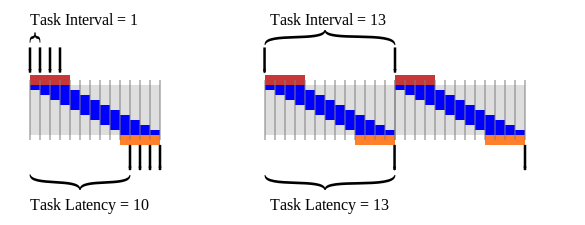
\includegraphics{intervalduration.pdf}
\caption{A block diagram showing a hypothetical embedded FPGA design, consisting of I/O interface cores (shown in blue), standard cores (shown in green), and application specific accelerator cores (shown in purple).  Note that accelerator cores might have streaming interfaces (Accelerator 2), memory-mapped interfaces (Accelerator 3), or both (Accelerator 1). }
\label{fig:designTemplate}
\end{figure}

Away from I/O pins, FPGA designs often contain \term{standard cores}, such as processor cores, on-chip memories, and interconnect switches.   Other standard cores include generic, fixed-function processing components, such as filters, FFTs, and codecs.  Although instances of these cores are often parameterized and assembled in a wide variety of ways in a different designs, they are not typically the differentiating element in a customers design.  Instead, they represent commodity, horizontal technology that can be leveraged in designs in many different application areas.   As a result, they are often provided by an FPGA vendor or component provider and only rarely implemented by a system designer.  Unlike interface I/O cores, standard cores are primarily synchronous circuits that require few constraints other than basic timing constraints specifying the clock period.  As a result, such cores are typically portable between FPGA families, although their circuit structure may still be highly optimized.

Lastly, FPGA designs typically contain customized, application-specific \term{accelerator cores}.  As with standard cores, accelerator cores are primarily synchronous circuits that can be characterized by a clock period timing constraint.  In contrast, however, they are almost inevitably constructed for a specific application by a system designer.  These are often the ``secret sauce'' and used to differentiate your system from others. Ideally a designer can quickly and easily generate high-performance custom cores, perform a design space exploration about feasible designs, and integrate these into their systems in a short timeframe. This book will focus on the development of custom cores using HLS in a fast, efficient and high performance manner.

When integrating a design as in Figure \ref{fig:designTemplate}, there are two common design methodologies.  One methodology is to treat HLS-generated accelerator cores just like any other cores.  After creating the appropriate accelerator cores using HLS, the cores are composed together (for instance, in a tool such as \vivado IP Integrator) along with I/O interface cores and standard cores to form a complete design.  This \term{core-based design methodology} is similar to the way that FPGA designs are developed without the use of HLS.  A newer methodology focuses on standard design templates or platforms, which combine a stable, verified composition of standard cores and I/O interface cores targeting a particular board. This \term{platform-based design methodology} enables a high-level programmer to quickly integrate different algorithms or \term{roles} within the interfaces provided by a single platform or \term{shell}.  It can also make it easier to port an accelerator from one platform to another as long as the shells support the same standardized interfaces.


\section{Design Optimization}
\label{sec:designOptimization}

\subsection{Performance Characterization}
\label{sec:designCharacterization}
Before we can talk about optimizing a design, we need to discuss the key criterion that are used to characterize a design.   The computation time is a particularly important metric for design quality.  When describing synchronous circuits, one often will use the number of clock cycles as a measure of performance.  However, this is not appropriate when comparing designs that have different clock rates, which is typically the case in HLS. For example, the clock frequency is specified as an input constraint to the \VHLS, and it is feasible to generate different architectures for the same exact code by simply changing the target clock frequency.  Thus, it is most appropriate to use seconds, which allows an apples-to-apples comparison between any HLS architecture. The \VHLS tool reports the number of cycles and the clock frequency. These can be used to calculate the exact amount of time that some piece of code requires to compute.

\begin{aside}
It is possible to optimize the design by changing the clock frequency. The \VHLS tool takes as input a target clock frequency, and changing this frequency target will likely result in the tool generating different implementations. We discuss this throughout the book. For example, Chapter \ref{sec:fir-performance} describes the constraints the are imposed on the \VHLS tool depending on the clock period. Chapter \ref{sec:fir-chaining} discusses how increasing the clock period can increase the throughput by employing operation chaining.
\end{aside}

We use the term \gls{task} to mean a fundamental atomic unit of behavior; this corresponds to a function invocation in \VHLS.  The \gls{task-latency} is the time between when a task starts and when it finishes.  The \gls{task-interval} is the time between when one task starts and the next starts or the difference between the start times of two consecutive tasks.  All task input, output, and computation is bounded by the task latency, but the start of a task may not coincide with the reading of inputs and the end of a task may not coincide with writing of outputs, particularly if the task has state that is passed from one task to the next.  In many designs, \gls{data-rate} is a key design goal, and depends on both the \gls{task-interval} and the size of the arguments to the function.

\begin{figure}
\centering
\def\svgwidth{\columnwidth}
\includesvg{intervalduration}
%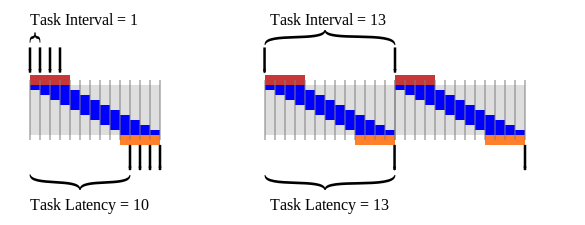
\includegraphics{intervalduration.pdf}
\caption{The task interval and task latency for two different designs. The left design is pipelined while the right one uses a more sequential implementation.}
\label{fig:intervalDuration}
\end{figure}

Figure \ref{fig:intervalDuration} shows two different designs of some hypothetical application.   The horizontal axis represents time (increasing to the right) and the vertical axis represents different functional units in the design.  Input operations are shaded red and and output operations are shaded orange.  Active operators are represented in dark blue and inactive operators are represented in light blue.  Each incoming arrow represents the start of a task and each outgoing arrow represents the completion of a task.  The diagram on the left represents four executions of an architecture that starts a new task every cycle. This corresponds to a `fully-pipelined' implementation. On the right, there is task with a very different architecture, reading a block of four pieces of input data, processing it, and then producing a block of four output samples after some time.  This architecture has the same latency and interval (13 cycles) and can only process one task at a time.  This behavior is in contrast to the behavior of the pipelined design on the left, which has multiple tasks executing at any given instant of time.  Pipelining in HLS is very similar to the concept of instruction pipelines in a microprocessor.  However, instead of using a simple 5-stage pipeline where the results of an operation are usually written back to the register file before being executed on again, the \VHLS tool constructs a circuit that is customized to run a particular program on a particular FPGA device.  The tool optimizes the number of pipeline stages, the initiation interval (the time between successive data provided to the pipeline -- similar to the task interval), the number and types of functional units and their interconnection based on a particular program and the device that is being targeted.

The \VHLS tool counts cycles by determining the maximum number of registers between any input and output of a task. Thus, it is possible for a design to have a task latency of zero cycles, corresponding to a combinational circuit which has no registers in any path from input to output. Another convention is to count the input and/or output as a register and then find the maximum registers on any path. This would result in a larger number of cycles. We use the \VHLS convention throughout this book.

\begin{aside}
Note that many tools report the task interval as ``throughput''. This terminology is somewhat counterintuitive since a longer task interval almost inevitably results in fewer tasks being completed in a given time and thus lower data rates at the interfaces.  Similarly, many tools use ``latency'' to describe a relationship between reading inputs and writing outputs.  Unfortunately, in designs with complex behavior and multiple interfaces, it is hard to characterize tasks solely in terms of inputs and outputs, e.g., a task may require multiple reads or writes from a memory interface. 
\end{aside}



% In general, Latency is additive with sequential composition, meaning that if a task $T_1$ passes data to a task $T_2$, then the combined latency is at least ${latency}(T_1)+{latency}(T_2)$.
%Most systems are pipelined, with a minimum initiation interval of 1 cycle.  Throughput is bounded by sequential composition, meaning that if a task $T_1$ feeds data to task $T_2$, then their throughput is ${max}({throughput}(T_1),{throughput}(T_2) )$

\subsection{Area/Throughput Tradeoffs}
\label{sec:filterThroughputTradeoffs}

In order to better discuss some of the challenges that one faces when using an HLS tool, let's consider a simple yet common hardware function -- the \gls{fir} (FIR) filter. An FIR performs a convolution on an input sequence with a fixed set of coefficients. An FIR is quite general -- it can be used to perform different types of filter (high pass filter, low pass, band pass, etc.).  Perhaps the most simple example of an FIR is a moving average filter. We will talk more background on FIR in Chapter \ref{chapter:fir} and describe many specific optimizations that can be done using HLS. But in the meantime just consider its implementation at a high level. 

The C code in Figure \ref{fig:FIR} provides a functional or task description for HLS; this can be directly used as input to the \VHLS tool, which will analyze it and  produce a functionally equivalent RTL circuit. This is a complex process, and we will not get into much detail about this now, but think of it as a compiler like gcc. Yet instead of outputting assembly code, the HLS ``compiler'' creates an RTL hardware description. In both cases, it is not necessary to understand exactly how the compiler works. This is exactly why we have the compiler in the first place -- to automate the design process and allow the programmer/designer to work at a higher level of abstraction. Yet at the same time, someone that knows more about how the compiler works will often be able to write more efficient code. This is particularly important for writing HLS code since there are many options for synthesizing the design that are not typically obvious to one that only knows the ``software'' flow. For example, ideas like custom memory layout, pipelining, and different I/O interfaces are important for HLS, but not for a ``software compiler''. These are the concepts that we focus on in this book.

A key question to understand is: ``What circuit is generated from this code?''.  Depending on your assumptions and the capabilities of a particular HLS tool, the answer can vary widely. There are multiple ways that this could be synthesized by an HLS tool. %To begin to understand the characteristics of HLS designs, we focus on the two implementations in Figures \ref{fig:FIR_sequential} and \ref{fig:FIR_function_pipeline}.

\begin{figure}
{
\lstinputlisting[format=none]{examples/fir.c}
%\begin{tikzpicture}[remember picture,overlay,>=stealth']
%\draw[<-,ultra thick] (pic cs:line-examples/fir.c-2-end) +(1em,.7ex) -| +(4,1em) node[above,comment,thin] {Comment};
%\end{tikzpicture}
}
\caption{Code for a four tap FIR filter.
}\label{fig:FIR}
\end{figure}

\begin{figure}
{
\hbox{\lstinputlisting{examples/fir.S}}\hbox{\includesvg{filter_asm_behavior}}
%\begin{tikzpicture}[remember picture,overlay,>=stealth']
%\draw[<-,ultra thick] (pic cs:line-examples/fir.c-2-end) +(1em,.7ex) -| +(4,1em) node[above,comment,thin] {Comment};
%\end{tikzpicture}
}
\caption{RISC-style assembly generated from the C code in Figure \ref{fig:FIR}, targetting the Xilinx Microblaze processor.  This code is generated using \texttt{microblazeel-xilinx-linux-gnu-gcc -O1 -mno-xl-soft-mul -S fir.c}}\label{fig:FIR_microblaze}
\end{figure}

One possible circuit would execute the code sequentially, as would a simple RISC microprocessor.  Figure \ref{fig:FIR_microblaze} shows assembly code for the Xilinx Microblaze processor which implements the C code in Figure \ref{fig:FIR}.  Although this code has been optimized, many instructions must still be executed to compute array index expressions and loop control operations.  If we assume that a new instruction can be issued each clock cycle, then this code will take approximately 49 clock cycles to compute one output sample of the filter.  Without going into the details of how the code works, we can see that one important barrier to performance in this code is how many instructions can be executed in each clock cycle.  Many improvements in computer architecture are fundamentally attempts to execute more complex instructions that do more useful work more often.  One characteristic of HLS is that architectural tradeoffs can be made without needing to fit in the constraints of an instruction set architecture.  It is common in HLS designs to generate architectures that issue hundreds or thousands of RISC-equivalent instructions per clock with pipelines that are hundreds of cycles deep.

By default, the \VHLS tool will generate an optimized, but largely sequential architecture.   In a sequential architecture, loops and branches are transformed into control logic that enables the registers, functional units, and the rest of the data path.  Conceptually, this is similar to the execution of a RISC processor, except that the program to be executed is converted into a finite state machine in the generated RTL rather than being fetched from the program memory.   A sequential architecture tends to limit the number of functional units in a design with a focus on resource sharing over massive parallelism.  Since such an implementation can be generated from most programs with minimal optimization or transformation, this makes it easy for users to get started with HLS.  One disadvantage of a sequential architecture is that analyzing and understanding data rates is often difficult since the control logic can be complex.  The control logic dictates the number of cycles for the task interval and task latencies. The control logic can be quite complex, making it difficult to analyze. In addition, the behavior of the control logic may also depend on the data being processed, resulting in performance that is data-dependent.

\begin{figure}
\centering
\mbox{\includesvg{filter_one_sample}}\mbox{\includesvg{filter_one_sample_behavior}}
\caption{A ``one tap per clock'' architecture for an FIR filter.  This architecture can be implemented from the code in Figure \ref{fig:FIR}.}
\label{fig:FIR_sequential}
\end{figure}

\begin{figure}
\centering
\mbox{\includesvg{filter_one_tap}}\mbox{\includesvg{filter_one_tap_behavior}}
%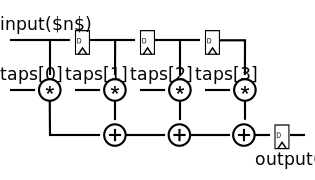
\includegraphics{filter_one_tap.pdf}
\caption{A ``one sample per clock'' architecture for an FIR filter.  This architecture can be implemented from the code in Figure \ref{fig:FIR} using function pipeline.}\label{fig:FIR_function_pipeline}
\end{figure}

However, the \VHLS tool can also generate higher performance pipelined and parallel architectures.  One important class of architectures is called a \term{function pipeline}.  A function pipeline architecture is derived by considering the code within the function to be entirely part of a computational data path, with little control logic.  Loops and branches in the code are converted into unconditional constructs.  As a result, such architectures are relatively simple to characterize, analyze, and understand and are often used for simple, high data rate designs where data is processed continuously.  Function pipeline architectures are beneficial as components in a larger design since their simple behavior allows them to be resource shared like primitive functional units.  One disadvantage of a function pipeline architecture is that not all code can be effectively parallelized.

The \VHLS tool can be directed to generate a function pipeline by placing the \lstinline|#pragma HLS pipeline| directive in the body of a function.  This directive takes a parameter that can be used to specify the initiation interval of the the pipeline, which is the same as a task interval for a function pipeline.  Figure \ref{fig:FIR_sequential} shows one potential design -- a ``one tap per clock'' architecture, consisting of a single multiplier and single adder to compute the filter.  This implementation has a task interval of 4 and a task latency of 4.  This architecture can take a new sample to filter once every 4 cycles and will generate a new output 4 cycles after the input is consumed. The implementation in Figure \ref{fig:FIR_function_pipeline} shows a ``one sample per clock'' architecture, consisting of 4 multipliers and 3 adders.  This implementation has a task interval of 1 and a task latency of 1, which in this case means that the implementation accept a new input value every cycle. Other implementations are also possible, such as architectures with ``two taps per clock'' or ``two samples per clock'', which might be more appropriate for a particular application.   We discuss more ways to optimize the FIR function in depth in Chapter \ref{chapter:fir}. 

In practice, complex designs often include complicated tradeoffs between sequential architectures and parallel architectures, in order to achieve the best overall design.  In \VHLS, these tradeoffs are largely controlled by the user, through various tool options and code annotations, such as \lstinline|#pragma| directive.

\begin{exercise}
What would the task interval of a ``two taps per clock'' architecture for a 4 tap filter be?  What about for a ``two samples per clock'' architecture?
\end{exercise}

\subsection{Restrictions on Processing Rate}

As we have seen, the task interval of a design can be changed by selecting different kinds of architectures, often resulting in a corresponding increase in the processing rate.  However, it is important to realize that the task interval of any processing architecture is fundamentally limited in several ways.  The most important limit arises from \glspl{recurrence} or feedback loops in a design.  The other key limitation arises from \term{resource limits}.

%\subsubsection{Recurrences}

A \term{recurrence} is any case where a computation by a component depends on a previous computation by the same component.  A key concept is that {\em recurrences fundamentally limit the throughput of a design}, even in the presence of pipelining \cite{papaefthymiou91,leiserson93}.  As a result, analyzing recurrences in algorithms and generating hardware that is guaranteed to be correct is a key function of an HLS tool.  Similarly, understanding algorithms and selecting those without tight recurrences is a important part of using HLS (and, in fact, parallel programming in general).

Recurrences can arrive in different coding constructs, such as static variables (Figure \ref{fig:FIR}), sequential loops (Figure \ref{fig:FIR_sequential}).  Recurrences can also appear in a sequential architecture and disappear when pipelining is applied (as in Figures \ref{fig:FIR_sequential} and \ref{fig:FIR_function_pipeline}).  In other cases, recurrences can exist without limiting the throughput of a sequential architecture, but can become problematic when the design is pipelined.

%\begin{figure}
%%\lstinputlisting{static_recurrence.cpp}
%\caption{A recurrence in a function, resulting from the use of \term{static} variables. \note{Need to add the code for this.}}
%\label{fig:static_recurrence.}
%\end{figure}

%\begin{figure}
%%\lstinputlisting{loop_recurrence.cpp}
%\caption{A recurrence in a function, as part of a loop. \note{Need to add the code for this.}}
%\label{fig:loop_recurrence}
%\end{figure}
%
%\note{Loops with array accesses are a particular case where HLS analyzes data dependencies...?}

%\subsubsection{Resource Limitations}

Another key factor that can limit processing rate are resource limitations.  One form of resource limitation is associated with the wires at the boundary of a design, since a synchronous circuit can only capture or transmit one bit per wire per clock cycle.  As a result, if a function with the signature \lstinline|int32_t f(int32_t x);| is implemented as a single block at 100 MHz with a task interval of 1, then the most data that it can process is 3.2 Gbits/sec. Another form of resource limitation arises from memories since most memories only support a limited number of accesses per clock cycle.  Yet another form of resource limitation comes from user constraints.  If a designer limits the number of operators that can instantiated during synthesis, then this places a limit on the processing rate of the resulting design.

%\subsection{Ordering Requirements}
%
%One key difference between a function pipelined architecture and a sequential architecture is that the processing order in a sequential architecture is implied by the structure of the loop.

\subsection{Coding Style}

Another key question you should ask yourself is, ``Is this code the best way to capture the algorithm?''.  In many cases, the goal is not only the highest quality of results, but maintainable and modifiable code.  Although this is somewhat a stylistic preference, coding style can sometimes limit the architectures that a HLS tool can generate from a particular piece of code.

For instance, while a tool might be able to generate either architecture in Figure \ref{fig:FIR_function_pipeline} or \ref{fig:FIR_sequential} from the code in Figure \ref{fig:FIR}, adding additional directives as shown in Figure \ref{fig:block_FIR} would result in a specific architecture. In this case the delay line is explicitly unrolled, and the multiply-accumulate \lstinline|for| loop is stated to be implemented in a pipelined manner. This would direct the HLS tool to produce an architecture that looks more like the pipelined one in Figure \ref{fig:FIR_function_pipeline}.

\begin{figure}
\lstinputlisting{examples/block_fir.c}
\caption{Alternative code implementing an FIR filter.}\label{fig:block_FIR}
\end{figure}



% In some applications, it is also advantageous to utilize other characteristics of the filter, such as symmetry to reduce the number of multipliers. 

\begin{exercise}
The chapter described how to build filters with a range of different processing rates, up to one sample per clock cycle.  However, many designs may require processing data at a higher rate, perhaps several samples per clock cycle.  How would you code such a design?  Implement a 4 samples per clock cycle FIR filter.  How many resources does this architecture require (e.g., number of multipliers and adders)? Which do you think will use more FPGA resources: the 4 samples per clock or the 1 sample per clock cycle design?  
\end{exercise}

We look further into the optimization of an FIR function in more detail in Chapter \ref{chapter:fir}. We discuss how to employ different optimizations (pipelining, unrolling, bitwidth optimization, etc.), and describe their effects on the performance and resource utilization of the resulting generated architectures.

\section{Restructured Code}

Writing highly optimized synthesizable HLS code is often not a straightforward process. It involves a deep understanding of the application at hand, the ability to change the code such that the \VHLS tool creates optimized hardware structures and utilizes the directives in an effective manner. 

Throughout the rest of the book, we walk through the synthesis of a number of different application domains -- including digital signal processing, sorting, compression, matrix operations, and video processing. In order to get the most efficient architecture, it is important to have a deep understanding of the algorithm. This enables optimizations that require rewriting the code rather than just adding synthesis directives -- a processing that we call code restructuring. 

%In this chapter, we walk through the synthesis of small examples, but ones that require a careful understanding of the \VHLS tool and restructuring the code in order to obtain good results. 

\term{Restructured code} maps well into hardware, and often represents the eccentricities of the tool chain, which requires deep understanding of micro-architectural constructs in addition to the algorithmic functionality. Standard, off-the-shelf code typically yields very poor quality of results that are orders of magnitude slower than CPU designs, even when using HLS directives such as pipelining, unrolling, and data partitioning. Thus, it is important to understand how to write code that the \VHLS will synthesize in an optimal manner.

Restructured code typically differs substantially from a software implementation -- even one that is highly optimized. A number of studies suggest that restructuring code is an essential step to generate an efficient FPGA
design \cite{mataidesigning, matai2energy, cong2011high, chen2012fpga, lee250high}. Thus, in order to get an efficient hardware design, the user must write restructured code with the underlying
hardware architecture in mind. Writing restructured code requires significant
hardware design expertise and domain specific knowledge. 

Throughout the rest of this book, we go through a number of different applications, and show how to restructure the code for a more efficient hardware design. We present applications such as finite impulse response (FIR), discrete Fourier transform (DFT), fast Fourier transform (FFT), sparse matrix vector multiply (SpMV), matrix multiplication, sorting, and Huffman encoding. We discuss the impact of restructured code on the final hardware generated from high-level synthesis. And we propose a restructuring techniques based on best practices. In each chapter, we aim to:
\begin{enumerate}
	\item Highlight the importance of restructuring code to obtain FPGA
          designs with good quality of result, i.e., a design that has high performance and low area usage;
	\item Provide restructured code for common applications;
	\item Discuss the impact of the restructuring on the underlying hardware; and
	\item Perform the necessary HLS directives to achieve the best design
\end{enumerate}
Throughout the book, we use example applications to show how to move from a baseline implementation and restructure the code to provide more efficient hardware design. We believe that the optimization process is best understood through example. Each chapter performs a different set of optimization directives including pipelining, dataflow, array partitioning, loop optimizations, and bitwidth optimization.  Additionally, we provide insight on the skills and knowledge necessary to perform the code restructuring process.

\section{Book Organization}
We organized this book to teach by example. Each chapter presents an application (or application domain) and walks through its implementation using  different HLS optimizations. Generally, each chapter focuses on a limited subset of optimization techniques. And the application complexity generally increases in the later chapters. We start with a relatively simple to understand finite impulse response (FIR) filter in Chapter \ref{chapter:fir} and move on to implement complete video processing systems in Chapter \ref{chapter:video}. 

There are of course benefits and drawbacks to this approach. The benefits are: 1) the reader can see how the optimizations are directly applicable to an application, 2) each application provides an exemplar of how to write HLS code, and 3) while simple to explain, toy examples can be hard to generalize and thus do not always make the best examples. 

The drawbacks to the teach by example approach are: 1) most applications requires some background to give the reader a better understanding of the computation being performed. Truly understanding the computation often necessitates an extensive discussion on the mathematical background on the application. For example, implementing the best architecture for the fast Fourier transform (FFT) requires that the designer have deep understanding of the mathematical concepts behind a discrete Fourier transform (DFT) and FFT. Thus, some chapters, e.g., Chapter \ref{chapter:dft} (DFT) and Chapter \ref{chapter:fft} (FFT), start with a non-trivial amount of mathematical discussion. This may be off-putting to a reader simply looking to understand the basics of HLS, but we believe that such a deep understanding is necessary to understand the code restructuring that is necessary to achieve the best design. 2) some times a concept could be better explained by a toy example that abstracts away some of the non-important application details. 

The organization for each chapter follows the same general pattern. A chapter begins by providing a background on the application(s) under consideration. In many cases, this is straightforward, e.g., it is not too difficult to explain matrix multiplication (as in Chapter \ref{chapter:matrix_multiplication}) while the DFT requires a substantial amount of discussion (Chapter \ref{chapter:dft}). Then, we provide a \emph{baseline implementation} -- a functionally correct but unoptimized implementation of the application using \VHLS. After that, we perform a number of different optimizations. Some of the chapters focus on a small number of optimizations (e.g., Chapter \ref{chapter:cordic} emphasizes bitwidth optimizations) while others look at a broad range of optimizations (e.g., Chapter \ref{chapter:fir} on FIR filters). The key optimizations and design methods are typically introduced in-depth in one chapter and then used repeatedly in the subsequent chapters. 

The book is made to be read sequentially. For example, Chapter \ref{chapter:fir} introduces most of the optimizations and the later chapters provide more depth on using these optimizations. The applications generally get more complex throughout the book. However, each chapter is relatively self-contained. Thus, a more advanced HLS user can read an individual chapter if she only cares to understand a particular application domain. For example, a reader interested in generating a hardware accelerated sorting engine can look at Chapter \ref{chapter:sorting} without necessarily have to read all of the previous chapters. This is another benefit of our teach by example approach.



\begin{table}[htp]
\caption{A map describing the types of HLS optimizations and the chapters that discuss the concepts beyond them.}
\begin{center}
\begin{tabular}{c||c|c|c|c|c|c|c|c|c|c|}
Chapter & \rotatebox{90}{FIR} & \rotatebox{90}{CORDIC} & \rotatebox{90}{DFT} & \rotatebox{90}{FFT} & \rotatebox{90}{SPMV} & \rotatebox{90}{MatMul} & \rotatebox{90}{Histogram} & \rotatebox{90}{Video} & \rotatebox{90}{Sorting} & \rotatebox{90}{Huffman} \\
 & 2 & 3 & 4 & 5 & 6 & 7 & 8 & 9 & 10 & 11 \\
\hline \hline
Loop Unrolling & X & & X & X & X & & X & & X &  \\
Loop Pipelining & X & & X & X & X & & X & X & X & X \\
Bitwidth Optimization & X & X & & & & & & & & X  \\
Function Inlining & X & & & & & & & & & X  \\
Hierarchy & X & & & X & & & X & X & X & X  \\
Array Optimizations &  & & X & X & X & X & X & X & X & X  \\
Task Pipelining &  & &  & X & & & X & X & X & X  \\
Testbench &  & & & & X & X & & & X & X  \\
Co-simulation &  & & & & X & & & & &  \\
Streaming &  & & & &  & X & & X & X &  \\
Interfacing &  & & & &  & & & X & &  \\

\end{tabular}
\end{center}
\label{table:optimizations}
\end{table}%

Table \ref{table:optimizations} provides an overview of the types of optimization and the chapters where they are covered in at least some level of detail. Chapter \ref{chapter:fir} provides a gentle introduction the HLS design process. It overviews several different optimizations, and shows how they can be used in the optimization of a FIR filter. The later chapters go into much more detail on the benefits and usage of these optimizations. 

The next set of chapters (Chapters \ref{chapter:cordic} through \ref{chapter:fft}) build digital signal processing blocks (CORDIC, DFT, and FFT). Each of these chapters generally focuses on one optimization: bitwidth optimization (Chapter \ref{chapter:cordic}), array optimizations (Chapter \ref{chapter:dft}, and task pipelining (Chapter \ref{chapter:fft}). For example, Chapter \ref{chapter:cordic} gives an in-depth discussion on how to perform bitwidth optimizations on the CORDIC application.  Chapter \ref{chapter:dft} provides an introduction to array optimizations, in particular, how to perform array partitioning in order to increase the on-chip memory bandwidth. This chapter also talks about loop unrolling and pipelining, and the need to perform these three optimizations in concert. Chapter \ref{chapter:fft} describes the optimizations of the FFT, which itself is a major code restructuring of the DFT. Thus, the chapter gives a background on how the FFT works. The FFT is a staged algorithm, and thus highly amenable to task pipelining. The final optimized FFT code requires a number of other optimizations including loop pipelining, unrolling, and array optimizations. Each of these chapters is paired with a project from the Appendix. These projects lead the design and optimization of the blocks, and the integration of these blocks into wireless communications systems. 

Chapters \ref{chapter:spmv} through \ref{chapter:huffman} provide a discussion on the optimization of more applications. Chapter \ref{chapter:spmv} describes how to use a testbench and how to perform RTL co-simulation. It also describes array and loop optimizations; these optimizations are common and thus are used in the optimization of many applications. Chapter \ref{chapter:matrix_multiplication} introduces the streaming optimization for data flow between tasks. Chapter \ref{chapter:prefixsum} presents two applications (prefix sum and histogram) that are relatively simple, but requires careful code restructuring in order to create the optimal architecture. Chapter \ref{chapter:video} talks extensively about how to perform different types interfacing, e.g., with a video stream using different bus and memory interfaces. As the name implies, the video streaming requires the use of the stream primitive, and extensive usage of loop and array optimizations. Chapter \ref{chapter:sorting} goes through a couple of sorting algorithms. These require a large number of different optimizations. The final chapter creates a complex data compression architecture. It has a large number of complex blocks that work on a more complex data structure (trees). 

%Unfortunately, there is no automatic process for identifying code optimization.  However, with practice and a little bit of creativity, w It typically takes an expert hardware designer with a deep understanding of the \VHLS tool. Like with any skill worth learning, practice makes perfect. 
%\subsection{Data-stationary vs. Processing-stationary programs}
%
%
%
%\subsection{Different kinds of pipelines}
%flushable vs stalling
%
%task pipelined vs not
%
%statically scheduled vs dynamically scheduled
%
%\subsection{Building Streaming Pipelines}
%\label{sec:streaming}
%
%Looking again at the 
%
%\subsection{Building Parameterizable Libraries}
